94. $y=\cfrac{|x^2-6x+8|}{x-2}=\cfrac{|x-2||x-4|}{x-2}=\begin{cases} |x-4|, x>2,\\ -|x-4|, x<2.\end{cases}=\begin{cases} x-4,\ x\geqslant 4,\\ 4-x,\ 2<x<4,\\ x-4,\ x<2.\end{cases}$
$$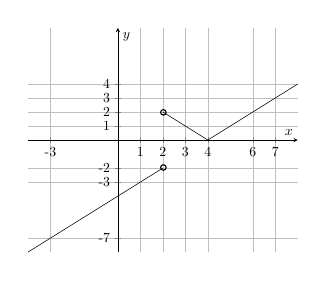
\begin{tikzpicture}[scale=0.5]
\begin{axis}[
    axis lines = middle,
    grid=major,
    legend pos={south west},
    xlabel = {$x$},
    ylabel = {$y$},
    ymin=-8,
    ymax=8,
    xtick={-3,1,2, 3,4,6,7},
    xticklabels={-3,1,2, 3,4,6,7},
    ytick={-7,-3,-2,1,2, 3,4},
    yticklabels={-7,-3,-2,1,2, 3,4}            ]
\addplot[domain=-4:2, samples=100, color=black] {-abs(x-4)};
\addplot[domain=2:8, samples=100, color=black] {abs(x-4)};
%\addplot[domain=-3.1:2.5, samples=100, color=red] {70*abs(1-2*abs(abs(x)-2))-10*x^2+10*x-70};
	%\addlegendentry{$\text{Рис. 1}$};
\end{axis}
\draw (3.44,3.55) circle (2pt);
\draw (3.44,2.15) circle (2pt);
\end{tikzpicture}$$\\
